% arara: lualatex: { draft: true }
% arara: lualatex: {interaction: nonstopmode , synctex: 1}

\documentclass[
ngerman,
ruledheaders=section,
class=report,
thesis={type=Dokumentation},
ignore-missing-data=true,
accentcolor=9c,
custommargins=false,
marginpar=false,
parskip=half-,
fontsize=11pt,
]{tudapub}

% compatibility with older pdflatex versions
\usepackage{iftex}
\ifPDFTeX
\usepackage[utf8]{inputenc}
\fi

% language packages
\usepackage[english, main=ngerman]{babel}
\usepackage[autostyle]{csquotes}

% tables
\usepackage{tabularx}
\usepackage{booktabs}

% mathematics
\usepackage{mathtools}
\usepackage{amssymb}
\usepackage{siunitx}
\sisetup{locale=DE}

% further packages
\usepackage[skip=10pt]{caption}
\usepackage{graphics,graphicx}
\usepackage[sf, SF]{subfigure}
\usepackage{listings}
\lstset{numbers=left, 
	numberstyle=\tiny, 
	numbersep=10pt, 
	frame=tlbr,
	framesep=5pt,
	backgroundcolor=\color{lightgray}, 
	xleftmargin=25pt, 
	xrightmargin=5pt, 
	showstringspaces=false,
	captionpos=b, 
	tabsize=4}
\usepackage{epstopdf}
\usepackage{float}

% custom commands
\let\file\texttt
\let\code\texttt
\let\tbs\textbackslash
\let\pck\textsf
\let\cls\textsf
\newcommand{\mr}[1]{\mathrm{#1}}
\def\code#1{\begin{small}\texttt{#1}\end{small}}

% start document
\setlength\intextsep{22pt}
\begin{document}
	
	\Metadata{
		title=2. Hausübung - MPI,
		author=Leon Bohmann, Jonathan Stollberg
	}
	
	\title{2. Hausübung - MPI}
	\author[]{Leon Bohmann (2493657) und Jonathan Stollberg (247775)}
	\submissiondate{\today}
	
	\maketitle
	\tableofcontents
	
	\chapter{Einführung}
	Auf die 1. Hausübung aufbauend werden in dieser Ausarbeitung weitere Methoden zur parallelen Berechnung von Hauptproblemen der linearen Algebra berechnet. Genauer sollen Matrizen-Multiplikationen beschleunigt werden, indem ihre Berechnung auf meherere Anwendungs-Instanzen aufgeteilt und mittels des Message Passing Interfaces (MPI) verknüpft wird. Zur Berechnung des Speedups werden sequentielle wie auch die vorher verwendeten beschleunigten Algorithmen herangezogen. Zuletzt, wird der Code auf dem Lichtenberg Hochleistungsrechner ausgeführt.
	
	Das implementierte Programm löst das folgende Problem:
	\begin{equation}
		\text{\textbf{C}}=\text{\textbf{A}}\text{\textbf{B}}
	\end{equation}
	
	\chapter{Sequentieller Algorithmus}
	Zur Vergleichbarkeit wird ein sequentieller Algorithmus implementiert, der das oben beschriebene Problem lösen kann:
	
	\begin{lstlisting}[language=java,label=alg_sequential,caption={Sequentieller Algorithmus zur Berechnung Matrix-Matrix-Produkte}]
   	solution = new short[m * m];
	
	// compute matrix-vector product
	for (int i = 0; i < m; i++) {
		for (int j = 0; j < m; j++) {
			for (int k = 0; k < m; k++) {
				solution[i * m + k] += A[i * m + j] * B[j * m + k];
			}
		}
	}
	\end{lstlisting}
	
	Zum weiteren Vergleich wurde auch ein einfacher paralleler Algorithmus aus der ersten Hausübung übernommen:
	\begin{lstlisting}[language=java,label=alg_parallel_stream,caption={Paralleler Algorithmus mit Streams-API}]			
	solution = new short[m * m];
	IntStream.range(0, m).parallel().forEach(i -> {
		for (int j = 0; j < m; j++) {
			for (int k = 0; k < m; k++) {
				solution[i * m + k] += A[i * m + j] * B[j * m + k];
			}
		}
	});
	\end{lstlisting}
	
	Um die Richtigkeit der durch Streams und MPI parallel berechneten Ergebnisse zu gewährleisten, werden diese am Ende eines jeden Programmdurchlaufs mit dem sequentiell berechneten Ergebnis abgeglichen.
	
	\chapter{Cannon-Algorithmus}
	Um die Matrix aufzuteilen und mit einzelnen Programm-Instanzen berechnen zu können, bedarf es einem passenden Algorithmus. Hierfür wurde der Cannon-Algorithmus implementiert, da dieser die parallele Berechnung mit mehreren Programm-Instanzen erlaubt. Die Besonderheit des Cannon-Algorithmus ist, dass die einzelnen Prozesse auf dedizierte Speicheradressen zugreifen und somit Adress-Blockierungen umgangen werden können.
	
	\paragraph{Ablauf}
	Beim Cannon-Algorithmus wird die zugrundeliegende Matrix reihen- beziehungsweise spaltenweise verschoben. Die einzelnen Prozesse arbeiten dann immer mit der Submatrix an ihren Koordinaten. Der Prozess 1 einer Matrix mit 3x3 Einträgen arbeitet dann immer mit der Submatrix an der Position (0,0). Nach jeder Iteration, also der Berechnung der Submatrizen aller Prozesse werden die Matrixeinträge zyklisch vertauscht (siehe \ref{fig:cannon-steps}).
	
	\begin{figure}[H]
		\centering
		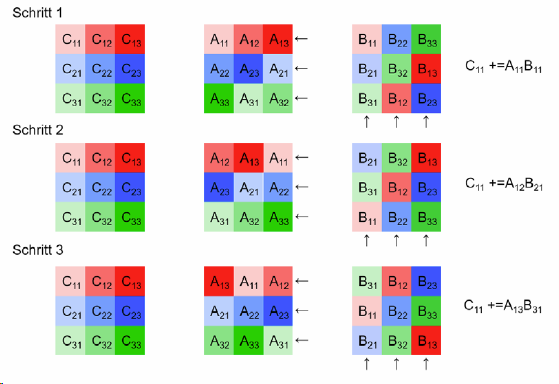
\includegraphics[width=0.7\linewidth]{content/cannon-steps}
		\caption{Zyklisches Vertauschen nach jeder Iteration}
		\label{fig:cannon-steps}
	\end{figure}
	
	In der darauf folgenden Iteration werden die neuen Daten an den Koordinaten des Prozesses von vorher verwendet und auf das Ergebnis summiert. Diese Operation kann man wie folgt formulieren:
	
	\begin{equation}
		\textbf{C}_{ij}=\sum_{n=0}^{size} \textbf{A}_{(il)} \cdot \textbf{B}_{(lj)}
	\end{equation}
	Durch die Klammern um die Indizes ist angedeutet, dass es sich um Submatrizen von $\textbf{A}$ und $\textbf{B}$ handelt. Die Besonderheit in der Formel ist (wie bereits erwähnt) in der Summation verborgen. Diese erfolgt nicht im Prozess $(i,j)$ sondern global für die zugrundeliegenden Matrizen $\textbf{A}$ und  $\textbf{B}$. Man erkennt aber leicht, dass die Formel analog der sequentiellen Matrizenmultiplikation ist. Angenommen, die Submatrizen sind Skalare, kann man die Formel also auch schreiben als:
	
	\begin{equation}
		\textbf{C}_{ij}=\sum_{l=0}^{n} \textbf{A}_{il}\textbf{B}_{lj}
		= \textbf{A}_{11}\textbf{B}_{11} + \textbf{A}_{12}\textbf{B}_{21} + \textbf{A}_{13}\textbf{B}_{31}
	\end{equation}
	
	Damit ist die Analogität leicht ersichtlich.
	
	\paragraph{Implementierung}
	Um die Matrix aufzuteilen muss zunächst die Anzahl an gleichzeitigen Prozessen sowie ihre jeweilige Kennung bestimmt werden. Dafür können die Message Passing Interface (MPI) Methoden \code{MPI.COMM\_WORLD.Rank()} und \code{MPI.COMM\_WORLD.Size()} verwendet werden. Mit den so bestimmten Größen können die Matrix-Blöcke definiert werden.
	
	Nun werden die Submatrizen an die einzelnen Prozesse verteilt. Dafür nutzt man die \code{MPI.COMM\_WORLD.Scatter(...)} Methode. Für eine korrekte Initialisierung des Algorithmus müssen die Submatrizen anschließend allerdings auf dem Prozessgitter zyklisch verschoben werden, wie in Abb.~\ref{fig:cannon-init} dargestellt. Die Submatrizen der Matrix $\textbf{A}$ werden zyklisch horizontal verschoben, die Submatrizen von $\textbf{B}$ vertikal.
	
	\begin{figure}[H]
		\centering
		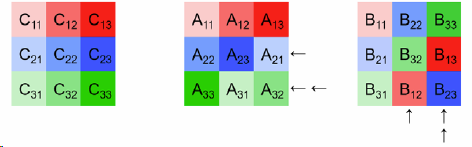
\includegraphics[width=0.7\linewidth]{content/cannon-init}
		\caption{Initialisierung des Algorithmus}
		\label{fig:cannon-init}
	\end{figure}
	
	Zur Realisierung der Verschiebungen nutzt man die \code{MPI.COMM\_WORLD.Sendrecv\_replace(...)} Methode bzw. alternativ die Methoden \code{MPI.COMM\_WORLD.Isend(...)} und \code{MPI.COMM\_WORLD.Irecv(...)}. Anschließend können die Submatrizen auf den jeweiligen Prozessen sequentiell miteinander multipliziert werden. Durch jede weitere Verschiebung bauen sich wie zuvor gezeigt die korrekten Submatrizen der Lösungsmatrix $\text{\textbf{C}}$ auf.
	
	Nach erfolgreicher Berechnung der Submatrizen kann das Ergebnis nun mittels \code{MPI.COMM\_WORLD.Gather(...)} wieder zurück in die globale Lösungs-Matrix geschrieben werden.
	
	\chapter{Zeitmessung}
	Die Zeitmessung wird von einem einzigen Prozess kontrolliert. Nachdem eine Barrieroperation alle laufenden MPI-Prozesse synchronisiert, misst dieser die Walltime. Melden alle Prozesse einen Abschluss, so wird erneut die Walltime erfasst und so die gesamte Berechnungsdauer ermittelt.
	
	\chapter{Benchmark und Fazit}	
	Auf dem Lichtenberg Hochleistungsrechner wurden die Algorithmen nacheinander ausgeführt. In den folgenden Darstellungen werden der sequentielle, durch Streams parallelisierte und der durch MPI parallelisierte Algorithmus gegenüber gestellt.
	
	\begin{figure}[H]
		\centering
		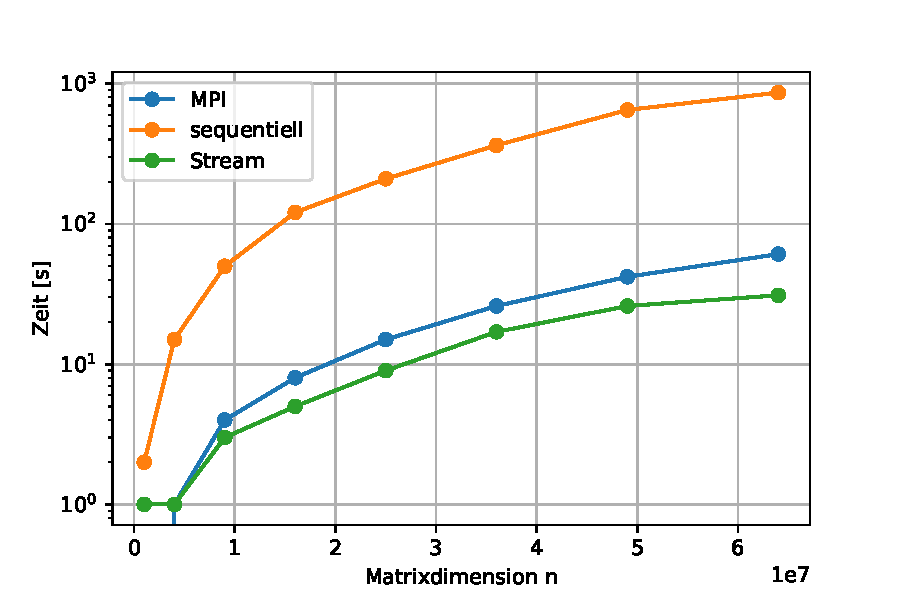
\includegraphics[width=0.7\linewidth]{content/16_procs_25000000}
		\caption{Berechnungsdauer in Abhängigkeit der Matrixdimension n, 16 Prozesse (bzw. Kerne)}
		\label{fig:16procs25000000}
	\end{figure}
	
	In \ref{fig:16procs25000000} ist die Berechnungsdauer einer Matrixmultiplikation bis 64 Mio. Einträgen dargestellt. Es ist zu erkennen, dass die parallelen Algorithmen um ein vielfaches schneller sind, als der Sequentielle. Auffälligt ist aber, dass die durch Streams realisierte Parallelisierung schneller ist, als die MPI-Methode. Das liegt vor allem daran, dass MPI eigentlich für mehrere Nodes zum Einsatz kommt. Dabei kann die Berechnung auf mehreren Rechnern mit wiederum mehreren Kernen ausgeführt werden, was im Rahmen dieser Versuche leider nicht möglich war, da auf dem Lichtenberg nur ein Knoten zur Verfügung stand. Außerdem ist der Zusatzaufwand der Datenverteilung durch MPI auf nur einem Knoten deutlich höher, als dass ihn der Speedup der eigentlich Berechnung wieder gut machen könnte.
		
	\begin{figure}[H]
		\centering
		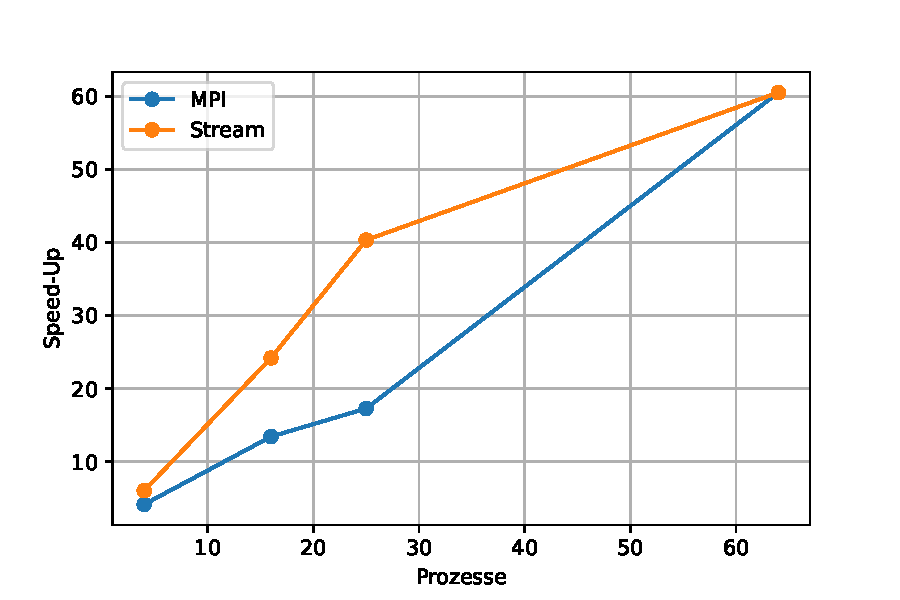
\includegraphics[width=0.6\linewidth]{content/speedup_16000000}
		\caption{Speedup gegenüber der sequentiellen Berechnung bei 16 Mio. Einträgen}
		\label{fig:speedup16000000}
	\end{figure}
	\begin{figure}[H]
		\centering
		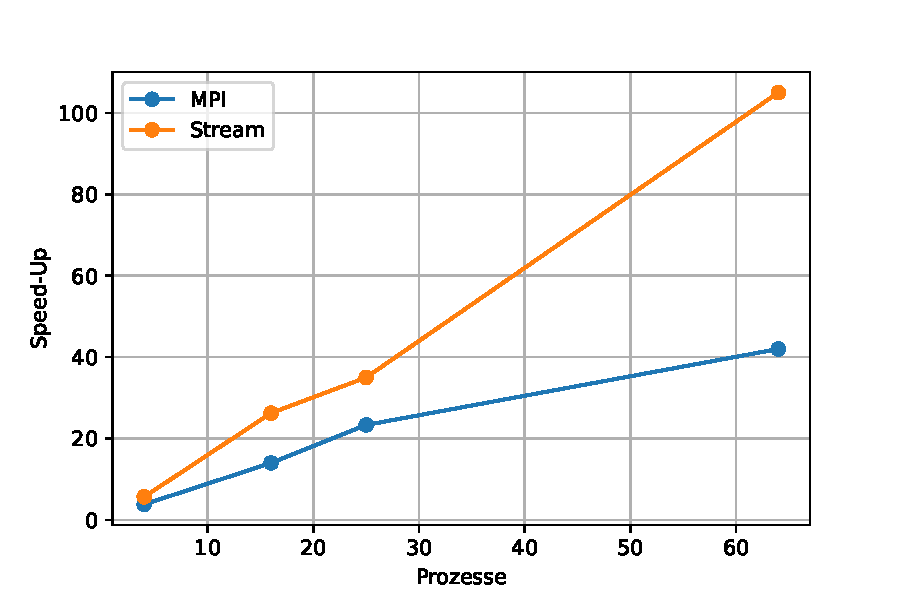
\includegraphics[width=0.6\linewidth]{content/speedup_25000000}
		\caption{Speedup gegenüber der sequentiellen Berechnung bei 25 Mio. Einträgen}
		\label{fig:speedup25000000}
	\end{figure}
	
	In \ref{fig:speedup16000000} und \ref{fig:speedup25000000} sind die relativen Speedups gegenüber der sequentiellen Berechnung dargestellt. Auffällig ist, dass die Berechnung der größeren Matrix mit Streams einen fast doppelt so großen Speedup erzielt als die der kleineren Matrix. Das deutet weiter darauf hin, dass die Datenverteilung durch MPI einen erheblichen Zeitaufwand birgt.
	
	Zusammenfassend kann festgehalten werden, dass die mögliche Beschleunigung durch die Verwendung von für MPI optimierte Parallelisierungen nicht ausgereizt werden konnte. Für einknotige Maschinen mit mehreren Kernen waren die durch Streams implementierten Algorithmen in jeder Hinsicht schneller und deutlich einfacher zu entwickeln.
	
\end{document}